\section{进阶要求：AscendNPU IR / MLIR 中端 lowering 探索}
\label{sec:advanced}
\subsection{实验目标与研究对象}
\label{subsec:multilevel-ir}
本部分研究同一 VecAdd 计算如何通过逐层 lowering 转换为面向 Ascend 设备的表示。LLVM IR 是相对单层的指令表示；MLIR 允许在多个抽象层次使用不同 dialect，通过 progressive lowering 逐步落实计算、存储与执行约束。本实验使用官方 AscendNPU IR VecAdd 示例，观察核类型推导、UB 内存规划、跨流水同步和模板转换如何在保留计算语义的同时补充设备相关信息。

实验采用 AscendNPU IR 1.1.0，其底层基于 LLVM 19.1.7；VecAdd 示例取自对应版本官方仓库\cite{ascendquick,bisheng,vecadd,ascendwheel}。编译器 pass 在 x86\_64 主机的 WSL 中运行，处理面向 Ascend 设备的 IR。示例直接以 HIVM 为入口：三个 \texttt{memref<16xi16>} 参数分别表示两个输入和一个输出，函数带有 DEVICE 属性。该工具链与基础实验的 LLVM 14 分开使用。


\subsection{同一计算的信息逐层显式化}
\label{subsec:lowering-information}
数学计算为 $C_j=A_j+B_j$，$j=0,\ldots,15$。原始 HIVM 给出 GM/UB 存储层次及整块 load、vadd、store；后续 pass 在保持计算语义的同时逐步补充执行约束。官方 host 源码将 A 初始化为 $0,\ldots,15$，B 全为 1，因此期望输出 C 为 $1,\ldots,16$。

为区分各阶段保留的计算语义与补充的执行约束，表\ref{tab:lowering}分别列出存储布局、核类型、同步和硬件特异信息。

\begin{table}[H]
\centering\footnotesize
\caption{IR 中逐步显式化的信息；每行保留前一行的约束}
\label{tab:lowering}
\setlength{\tabcolsep}{4pt}
\begin{tabularx}{\textwidth}{L{1.8cm}L{1.9cm}L{2.75cm}L{1.1cm}L{2.15cm}Y}
\toprule\rowcolor{tableHead}阶段 & 数学语义 & 存储层次 / 布局 & 核类型 & 同步 & 硬件特异信息 \\
\midrule
原始 HIVM & \mbox{$C=A+B$}，i16 & GM/UB；三个逻辑分配 & 未标注 & 无显式事件 & 16 元素 tile、设备函数 \\
核类型推导 & 同上 & 同上 & AIV & 同上 & 向量核约束显式化 \\
内存规划 & 同上 & UB 偏移 0、32、0；A/C 原地复用 & AIV & 同上 & 逻辑缓冲落实为地址 \\
同步插入 & 同上 & 同上 & AIV & 两对 set/wait；PIPE\_ALL & MTE2、V、MTE3 依赖 \\
模板转换 & 同上，由调用承接 & 地址空间及布局保留；转换 memref 接口 & AIV & 事件保留 & 三类设备模板的四次调用 \\
\bottomrule
\end{tabularx}
\end{table}

MLIR 多层表示的价值在于\textbf{让分析所需的语义保留到相应决策完成}：整块算子的输入/输出供活跃性和原地复用分析，存储层次与流水类别供同步分析，最后才转为后端模板调用。LLVM IR 也可表达地址空间和专用 intrinsic；本例采用较高层表示，直接保留 tile 与硬件操作结构，以便在拆分为低层操作前完成这些分析。

\subsection{从 use-def 到 UB 原地复用}
\label{subsec:ub-reuse}
每个 tile 占 $16\times2=32$ 字节。内存规划后的 IR 将 A、B、C 对应的 \texttt{pointer\_cast} 分别置于 UB 偏移 0、32、0。图\ref{fig:vecadd-lifetime}将逻辑数据流与\emph{缓冲内容}的活跃区间对应起来；它不同于 \texttt{memref.alloc} 结果作为 SSA 句柄的存在区间。

\begin{figure}[H]
\centering
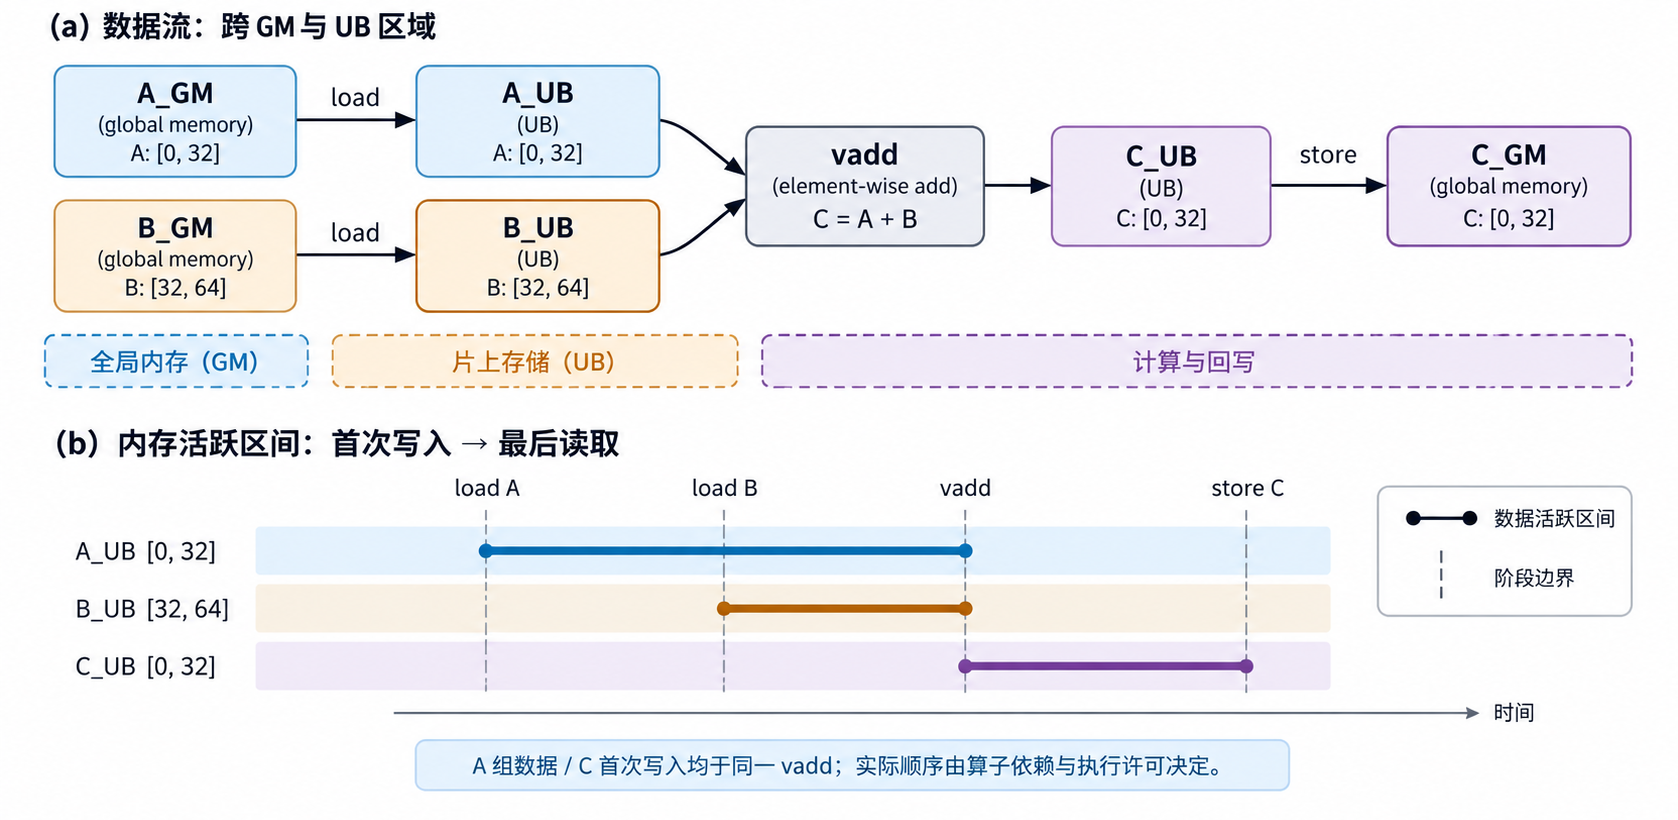
\includegraphics[width=\textwidth]{figures/fig6.png}
\caption{VecAdd 数据流和缓冲内容生命周期。区间为 UB 字节范围，横轴表示操作顺序。A 与 C 使用同一区域，并在 vadd 处共同活跃。}
\label{fig:vecadd-lifetime}
\end{figure}

A\_UB 的首次写入是 load A，最后一次读取是 vadd；B\_UB 同理。C\_UB 的首次写入也在\textbf{同一条 vadd}，最后读取是 store。在操作粒度上，输入的最后读取与输出的首次写入相遇，因此 A/C 共址的安全性还依赖该算子允许输入与输出原地重叠。

\texttt{PlanMemory.cpp}\cite{ascendplan}中，\texttt{IsReuseHIVMOp} 将无内联广播/转置的 VAdd 列入 ISA 允许原地执行的操作；\texttt{GenerateInplaceList} 在\emph{同一操作}的 gen/kill 集合中配对，要求被复用缓冲容量不小于新结果；\texttt{MergeInplaceSE} 在地址分配前合并相应存储条目。源码还检查操作数的 memref \emph{布局偏移}兼容性，这不同于最终规划的 UB 起始地址。本例具有相同形状和元素类型、各 32 字节、无广播/转置，且原 A 在 vadd 后不再读取，符合该原地复用路径。

由 use-def 关系、操作顺序及算子许可可知，本例 vadd 消费 A 后，以 C 替代其内容。上述原地复用结论仅针对本例 VAdd。静态布局使用 \texttt{[0,32)}、\texttt{[32,64)} 两段区域，相对三段独立缓冲由 96 字节减少为 64 字节；64 B 为静态 UB 布局结果，不代表设备运行时峰值或性能。偏移 0 以 UB 地址空间为基准。

\subsection{跨流水同步：从源文件顺序到 happens-before}
\label{subsec:cross-pipeline-sync}
本例 load 的 GM 至 UB 搬运属于 MTE2，vadd 属于 V，store 的 UB 至 GM 搬运属于 MTE3。它们是不同硬件流水线；IR 中 load 位于 vadd 之前，仍需同步操作保证向量流水在搬运完成后才消费数据。同步插入后的 IR 增加两对事件和末尾屏障，图\ref{fig:vecadd-pipeline}展示其依赖关系。

\begin{figure}[H]
\centering
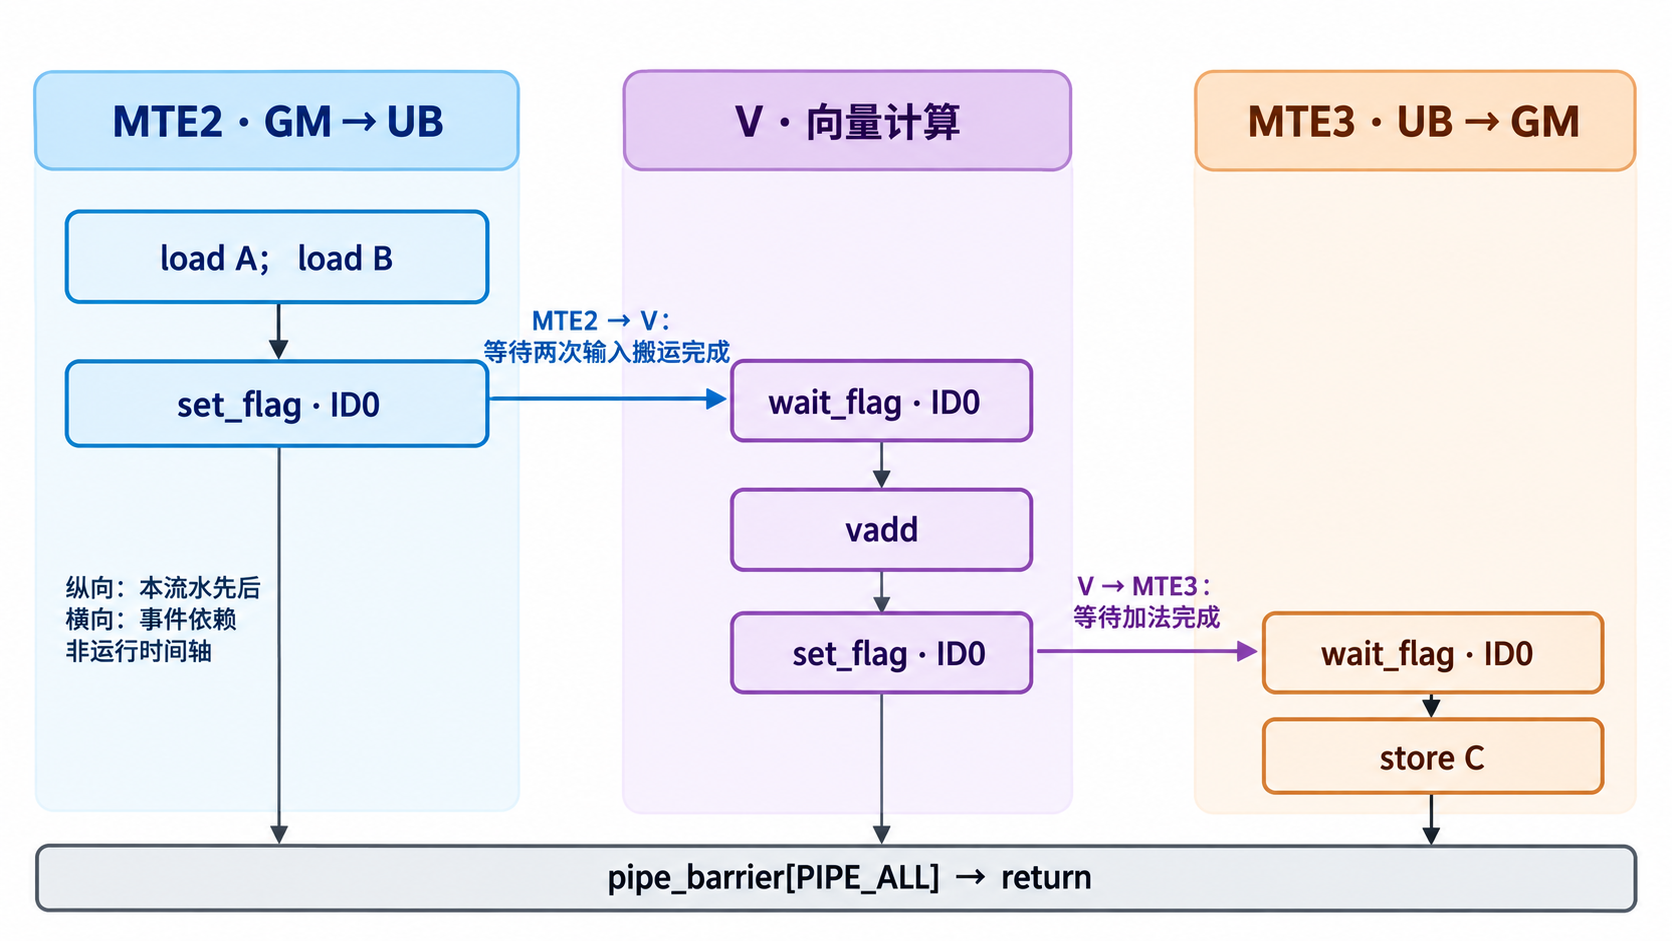
\includegraphics[width=\textwidth]{figures/fig7.png}
\caption{set/wait 配对形成的 happens-before。箭头表示流水线操作必须满足的先后关系。}
\label{fig:vecadd-pipeline}
\end{figure}

官方同步语义\cite{ascendsync}规定，\texttt{set\_flag} 等源流水前序指令完成后触发事件，\texttt{wait\_flag} 在目标流水阻塞后续指令直至事件触发。因此第一对建立“两次 load 完成 $\rightarrow$ vadd 可执行”，第二对建立“vadd 完成 $\rightarrow$ store 可执行”。两对均为 EVENT\_ID0，事件身份还包含源/目标流水：第一对为 MTE2$\rightarrow$V，第二对为 V$\rightarrow$MTE3。末尾 \texttt{pipe\_barrier[PIPE\_ALL]} 对核内所有流水施加前序完成约束，在返回处收束未完成工作；该屏障同步核内流水线，不承担多核全局同步。

\clearpage
\subsection{实际 pass 次序及其机制依赖}
\label{subsec:pass-order}
完整驱动的 \texttt{--mlir-print-ir-after-all} 输出显示以下关键顺序：核推导 $\rightarrow$ 全局 workspace 规划 $\rightarrow$ 局部 UB 规划 $\rightarrow$ \texttt{graph-sync-solver} $\rightarrow$ HIVM 模板转换；这里省略了中间其他 pass。两次 \texttt{plan-memory} 的职责不同，后一次在本例中将三个 alloc 变为 UB 偏移 0、32、0。\texttt{HIVMPipelines.cpp}\cite{ascendpipeline}中的全局规划模式、局部规划、随后同步调用及末尾模板转换与该顺序一致。

这一顺序体现了分析间的信息依赖：核推导根据设备操作约束明确 AIV，供后续设备变换使用；内存规划把逻辑缓冲落实为物理区域，使原地别名关系显式化；同步分析随后约束这些存储访问在各流水间的顺序；最后模板转换将搬运和向量操作的高层接口降为模板调用。核类型信息为设备变换提供约束，确定后的布局为同步处理提供存储访问关系。

逐步处理使用 \texttt{hivm-inject-sync}，完整驱动使用 \texttt{hivm-graph-sync-solver}；源码按选项分支选择二者。本例两条路径均产生上述关键依赖。五个逐步处理命令（含解析）与独立完整中端命令共完成六次处理，IR 重解析与关键结构一致性等 18 项检查均通过。

\subsection{模板 lowering 与后端边界}
\label{subsec:template-backend}
模板转换将两个 load、一个 vadd、一个 store 降为三类模板的四次调用：\path{load_gm_to_ubuf_1d_int16_t}、\path{vadd_1d_int16_t}、\path{store_ubuf_to_gm_1d_int16_t}。类型、实参与模板选择承接原计算；动态形状/步长的 \texttt{memref.cast} 调整调用接口。额外的第四个 \texttt{pointer\_cast} 是 vadd 的零长度临时缓冲参数，并非另一段有效数据存储。结果仍含 \texttt{func/arith/memref} 和 HIVM 同步、地址空间，\textbf{不是纯 LLVM IR}。

独立完整中端输出与驱动最终打印的模块一致。完整设备编译在外部 \texttt{hivmc} 处报告 \texttt{Cannot find hivmc under \$PATH}，\textbf{返回码为 0，且未产生 kernel.o}。驱动源码在外部后端失败后仍返回模块\cite{ascenddriver}，因此返回码 0 只反映驱动结束状态，设备编译结果还取决于诊断和目标文件。官方 host 示例仅打印 success，未逐元素校验输出。由于本地缺少 CANN/hivmc 与昇腾设备\cite{ascendfaq}，本实验完成了设备中端变换，设备 kernel 尚未生成，设备端数值正确性与性能尚未验证。

